%TODO
%	Procurar protocolos de gerencia especificos pra IoT
%
%	Capitulo de Gerencia de Redes com um viés mais IoT.
%
%	Na parte de gerência justificar a escolha do snmp por ser um padrão e 
% argumentar que é importante usá-lo para aproveitar a infraestrutura já 
% existente.
%
%	Comparar os protocolos de gerencia especificos pra IoT e dar enfase aos 
% pros e contras de cada um e entrar com a minha proposta pra melhorar esses 
% pontos.
%
%=======================================================================
% Declarações iniciais identificando a classe de documento e
% selecionando alguns pacotes adicionais.
%
% As opções disponíveis (separe-as com vírgulas, sem espaço) são:
% - twoside: Formata o documento para impressão frente-e-verso
%   (o default é somente-frente)
% - english,brazilian,french,german,etc.: idiomas usados no documento.
%   Deve ser colocado por último o idioma principal.
%=======================================================================
\documentclass[twoside,english,brazilian]{UNISINOSmonografia}
\usepackage[utf8]{inputenc} % charset do texto (utf8, latin1, etc.)
\usepackage[T1]{fontenc} % encoding da fonte (afeta a sep. de sílabas)
\usepackage{graphicx} % comandos para gráficos e inclusão de figuras

\usepackage{bibentry} % para inserir refs. bib. no meio do texto
\usepackage{hyperref}



\hypersetup{
	breaklinks=true,
	unicode=true,          % non-Latin characters in Acrobat’s bookmarks
	hidelinks=true,
	linktoc=all,
	pdflang=pt-BR
}

\graphicspath{ {./images/} }

%\hypersetup{
%	pdftitle={titulo},    % title
%	pdfauthor={mateus},     % author
%	pdfsubject={subsubsub},   % subject of the document
%	pdfkeywords={kkk1} {key2} {key3}, % list of keywords
%}
%=======================================================================
% Escolha do sistema para geração de referências bibliográficas.
%
% O default é usar o estilo unisinos.bst.  Comente a definição abaixo
% e descomente a linha seguinte para usar o estilo do ABNTeX (é
% necessário ter esse pacote instalado).
%
% A vantagem do unisinos.bst é que ele permite o uso de um arquivo .bib
% seguindo as orientações tradicionais do BibTeX (veja essas orientações
% em http://ctan.tug.org/tex-archive/biblio/bibtex/contrib/doc/btxdoc.pdf).
% Entretanto, o estilo não suporta algumas citações mais exóticas como
% apud.  Para isso, use o ABNTeX, mas esteja ciente de que muitas de
% suas referências serão incompatíveis com os estilos tradicionais do
% BibTeX como plain, alpha, ieeetr, entre outros.
%=======================================================================
\unisinosbst
%\usepackage[alf]{abntcite}



%=======================================================================
% Dados gerais sobre o trabalho.
%=======================================================================
\autor{Aubin}{Mateus Rauback}
\author{Mateus Rauback Aubin}
\titulo{
Um Sistema de Gestão de Dispositivos Inteligentes 
Baseado em Protocolos de Gerência de Redes Voltado Para a 
Internet das Coisas
}
%\subtitulo{Versão \LaTeX}
\orientador[Prof.~Dr.]{Ávila}{Rafael Bohrer}
%\coorientador[Prof.~Dr.]{Lamport}{Leslie}
\local{São Leopoldo}
\ano{2013}

%% dados específicos para monografia de Graduação
\unidade{Unidade Acadêmica Graduação}
\curso{Curso de Bacharelado em Ciência da Computação}
\natureza{
Trabalho de Conclusão de Curso apresentado como requisito parcial
para a obtenção do título de Bacharel em Ciência da Computação
pela Universidade do Vale do Rio dos Sinos --- Unisinos
}


%=======================================================================
% Palavras Chave.
%
% Deve ser fornecida para cada idioma.
%=======================================================================
\palavrachave{brazilian}{Internet das Coisas}
\palavrachave{english}{Internet of Things}

\palavrachave{brazilian}{Gerência de Redes}
\palavrachave{english}{Network Management}

\palavrachave{brazilian}{Protocolos de Rede}
\palavrachave{english}{Network Protocols}


%=======================================================================
% Início do documento.
%=======================================================================
\begin{document}	
\capa
\folhaderosto

%=======================================================================
% Dedicatória (opcional).
%
% O texto é normalmente colocado na parte de baixo da página, alinhado
% à direita.  Mas a formatação é basicamente livre.  Só não se escreve
% a palavra 'dedicatória'.
%=======================================================================
%\begin{dedicatoria}
%Aos nossos pais.\\[4ex] % quebra a linha dando um espaçamento maior
%\begin{itshape} % faz o texto ficar em itálico
%If I have seen farther than others,\\
%it is because I stood on the shoulders of giants.\\
%\end{itshape}
%--- \textsc{Sir Isaac Newton} % \textsc é o "small caps"
%\end{dedicatoria}


%=======================================================================
% Agradecimentos (opcional).
%=======================================================================
%\begin{agradecimentos}
%Obrigado!
%\end{agradecimentos}


%=======================================================================
% Epígrafe (opcional).
%
% ``[...] o autor apresenta uma citação, seguida de indicação de autoria,
% relacionada com a matéria tratada no corpo do trabalho. Podem, também,
% constar epígrafes nas folhas de aberturas das seções primárias.''
%=======================================================================
%\begin{epigrafe}
%``\textit{Ninguém abre um livro sem que aprenda alguma coisa}''.\\
%(Anônimo)
%\end{epigrafe}


%=======================================================================
% Resumo em Português.
%
% A recomendação é para 150 a 500 palavras.
%=======================================================================
%\begin{abstract}
%	Dica para elaborar um bom resumo: ele tem que responder às seguintes 
%questões:
%	- o que? (contexto)
%	- por que? (motivação)
%	- para que? (objetivos)
%	- como? (metodologia)
%\end{abstract}


%=======================================================================
% Resumo em língua estrangeira (obrigatório somente para teses e
% dissertações).
%
% O idioma usado aqui deve necessariamente aparecer nos parâmetros do
% \documentclass, no início do documento.
%=======================================================================
%\begin{otherlanguage}{english}
%\begin{abstract}
%Abstract goes here
%\end{abstract}
%\end{otherlanguage}


%=======================================================================
% Lista de Figuras (opcional).
%=======================================================================
%\listoffigures


%=======================================================================
% Lista de Tabelas (opcional).
%=======================================================================
%\listoftables


%=======================================================================
% Lista de Abreviaturas (opcional).
%
% Deve ser passada como parâmetro a maior das abreviaturas utilizadas.
%=======================================================================
%\begin{listadeabreviaturas}{seg., segs.}
%\item[ampl.] ampliado, -a
%\item[atual.] atualizado, -a
%\item[coord.] coordenador
%\item[N.~T.] Novo Testamento
%\item[seg., segs.] seguinte, -s
%\end{listadeabreviaturas}


%=======================================================================
% Lista de Siglas (opcional).
%
% Deve ser passada como parâmetro a maior das siglas utilizadas.
%=======================================================================
\begin{listadesiglas}{M2M}
\item[IoT] Internet of Things
\item[M2M] Machine-To-Machine
\item[TI] Tecnologia da Informação
\item[IP] Internet Protocol
\item[IPv6] Internet Protocol version 6
%\item[CAPES] Coordenação de Aperfeiçoamento de Pessoal de Nível Superior
%\item[FAPERGS] Fundação de Amparo à Pesquisa do Estado do Rio Grande do Sul
\end{listadesiglas}


%=======================================================================
% Lista de Símbolos (opcional).
%
% Deve ser passado o maior (mais largo) dos símbolos utilizados.
%=======================================================================
%\begin{listadesimbolos}{Ca}
%\item[\textsuperscript{o}C] Graus Celsius
%\item[Al] Alumínio
%\item[Ca] Cálcio
%\end{listadesimbolos}


%=======================================================================
% Sumário
%=======================================================================
\tableofcontents


%=======================================================================
% Introdução
%=======================================================================
\chapter{Introdução}

% as epígrafes nos capítulos são opcionais
\epigrafecap{
	In the nineteenth century, machines learned to do; in the twentieth 
	century, they learned to think; and in the twenty-first century, they are 
	learning to perceive -- they actually sense and respond.
}{\citetexto{Sundmaeker2010}}

%	Deve conter:
%		Apresentação do Assunto: IoT
%		Delimitação do Assunto:  Gerência de Redes aplicada a IoT
%		Justificativa:           Porque vai mudar a vida cotidiana
%		Localizar no Tempo:      Trabalhos de IoT
%		Ressaltar a Importância: Igual justificativa
%		Apresentar Objetivos:    Vide proposta
%		Apresentar a Estrutura:  Fica pro final
%		Explicar a Metodologia:  Vai ter capítulo específico

	Desde a Revolução Industrial há uma crescente busca pela automação das 
	tarefas humanas. Através de máquinas cada vez mais sofisticadas foi 
	possível obter significativo avanço nas tecnologias e nos métodos de 
	produção ao passo que diversas tarefas deixaram de ser realizadas 
	manualmente.
	Seguindo esta filosofia, máquinas computacionais foram projetadas e as 
	bases da ciência da computação estabelecidas. Conceitos como a 
	Álgebra Booleana de \citetexto{boole2003}, publicado originalmente em 
	1854, servem até hoje como fundamentos deste campo de estudos.

	Durante a segunda guerra mundial houve um expressivo progresso na 
	computação graças ao incentivo das organizações de defesa para melhorar 
	métodos de cálculo e criptografia. Neste período publicações como as de 
	\citetexto{Shannon1948}, \citetexto{Turing1937} e 
	\citetexto{VonNeumann1945} definiram a ciência da computação como é 
	conhecida hoje.

	Ainda com objetivos de defesa, pesquisas no campo de redes de computadores 
	começaram a ser desenvolvidas nos anos que seguiram. A IBM, nos anos 50,
	desenvolveu para os EUA o SAGE\footnote{Semi-Automatic Ground Environment, 
	um sistema nacional de defesa do espaço aéreo e um dos mais importantes 
	projetos da IBM. 
	\urlbr{set.~2013}{www.ibm.com/ibm/history/ibm100/us/en/icons/sage/}}, 
	um dos primeiros exemplos de computadores conectados em rede, 
	caracterizado pela ``transmissão de dados digitais em linhas telefônicas 
	de voz à 1300 bits por segundo'' \cite{IBMSAGE1983}.

	Contudo, o SAGE comunicava-se através do conceito de circuitos, que, mais 
	tarde, mostrou-se inferior à troca de pacotes (\textit{packet switching}). 
	Explorado pela agência de defesa americana nos anos 70, a comunicação via 
	troca de pacotes originou a ARPANET, uma rede nacional descentralizada 
	utilizada para interligar universidades e centros de pesquisas 
	\cite{ARPANET1964}, assim como os protocolos TCP/IP, a base da atual 
	internet.

	A contínua ampliação da capacidade de processamento dos dispositivos 
	computacionais, aliada a redução de custos, possibilitou uma nova 
	revolução tecnológica \cite{Atzori2010b}, abrindo caminho para a Era da 
	Informação.
	Munidos de circuitos integrados e \textit{microchips}, os computadores 
	estão cada vez mais presentes nas atividades humanas, avançando em direção 
	à ubiquidade.
	
	No atual cenário tecnológico já é possível, de maneira economicamente 
	viável, colocar em prática algumas das ideias vislumbradas por 
	\citetexto{Weiser1991}. 
	Apesar de representar um desafio para diversas áreas do conhecimento, as 
	barreiras para a efetiva integração entre dispositivos computacionais e a 
	vida cotidiana têm diminuído, possibilitando a criação de novos produtos e 
	serviços, resultando em soluções para os mais diversos problemas.
	
	Ainda que não seja uma proposta nova, \citetexto{Turck2013} pontua que a 
	implementação de uma rede composta de dispositivos embarcados em objetos 
	do dia-a-dia, ou seja, a Internet das Coisas (IoT), não era viável devido 
	a fatores como complexidade e custo. 
	Entretanto, tomando por referência a lei de \citetexto{Moore1965}, a qual 
	dita que o número de transístores em um circuito integrado dobra 
	aproximadamente a cada dois anos, é improvável que se reverta a tendência 
	de dispositivos cada vez menores e mais baratos, se reverta.
	
	Diversas são as semelhanças entre a Internet das Coisas e as Redes de 
	Sensores sem Fio, porém, enquanto as redes de sensores  
	são implantadas principalmente com o intuito de monitorar variáveis em um 
	ambiente \cite{Sakthidharan2012}, a Internet das Coisas expande este 
	conceito ao próximo nível. 
	A capacidade de tornar cada dispositivo individualmente endereçável na 
	internet favorece o compartilhamento de informações entre sistemas, 
	resultando em uma modalidade de comunicação chamada pela 
	\citetexto{ETSI2010} de comunicação Máquina-a-Máquina (M2M).
	
	Motivados pelas oportunidades e pelo alto impacto social da computação 
	pervasiva, impulsionada com a ajuda da IoT, pesquisadores tanto da 
	academia quanto da indústria se mobilizaram em torno deste conceito 
	\cite{Atzori2010b}. 
	Entidades governamentais reconheceram também a IoT como um paradigma 
	promissor, fomentando iniciativas de pesquisa e desenvolvimento em países 
	como China, Japão, Estados Unidos e da União Europeia 
	% p 16
	\cite{Sundmaeker2010}.
	
	Entretanto, com grandes poderes vêm grandes responsabilidades
	\footnote{Lição dada a Peter Parker por seu tio Ben na história em 
	quadrinhos Homem-Aranha, escrita por Stan Lee.}. 
	Para realizar sua visão, a Internet das Coisas deve superar uma série de 
	desafios, entre eles: privacidade, padronização tecnológica e 
	escalabilidade \cite{Coetzee2011}. 
	Para tanto, a cooperação entre academia, indústria e governo é fundamental 
	para que a IoT possa demonstrar seu verdadeiro potencial.
	
%TODO Apresentar a estrutura do trabalho (no cap x falaremos de IoT, no cap Y 
%		de Gerência, tal tal e tal)

\section{Justificativa e Definição do Problema}
%	Abordar
%		Justificativa: Porque com um monte de dispositivos espalhados por aí 
%		               vai ser difícil gerenciá-los um a um
%		Problema: Como fazer isso remotamente? Como fazer isso de maneira 
%		          padronizada? Como reaproveitar tecnologias estabelecidas?
%		Objetivo: Para facilitar a gestão de dispositivos inteligentes

	Em um mundo cada vez mais conectado e dependente da internet, a quantidade 
	de dispositivos capazes de integrar a rede já representa uma fatia 
	considerável entre os aparelhos usados diariamente \cite{Accenture2012}.
	Computadores, \textit{laptops}, \textit{tablets}, \textit{smartphones} e 
	televisores integram uma crescente classe de produtos comercialmente 
	chamados de Dispositivos Inteligentes (\textit{Smart Devices}) e que 
	permitem, dentre outras funções, acesso a redes e, consequentemente, à 
	internet.
	
	Paralelamente a esta tendência e seguindo as previsões de 
	\citetexto{Gilder2007} e \citetexto{Moore1965}, por exemplo, a capacidade 
	de equipamentos e redes continua a aumentar, resultando na visão de um 
	atraente e economicamente viável mundo conectado \cite{Ding2009}.
	Tais mudanças influenciam direta e indiretamente a sociedade, seus 
	costumes, e, conforme afirma \citetexto{Carr2010}, até mesmo o pensamento 
	humano.
	
	A difusão de aparelhos capazes de acessar a internet criou um novo 
	paradigma que está transformando a gestão de Tecnologia da Informação (TI) 
	\cite{ZdnetBYOD}.
	Este aumento apresenta-se como um desafio para as áreas de segurança da 
	informação e gerência de redes, convidando grandes empresas como 
	\citetexto{CiscoBYOD}, \citetexto{HP2013} e \citetexto{Motorola2011} a 
	propor novas soluções.
	
	Apesar de constituir um desafio de gestão, não há indícios da redução de 
	dispositivos nas redes. A Internet das Coisas trará consigo uma vasta gama 
	de novos aparelhos que carecem de diretivas de gestão \cite{Atzori2010b} 
	e, ainda que novas soluções estejam em desenvolvimento, não há um acordo 
	sobre mecanismos específicos de gerência, resultando em soluções 
	proprietárias e que não colaboram entre si.
	
	Visando manter a interoperabilidade entre dispositivos, há, nas pesquisas 
	de IoT, um consenso referente ao uso do Protocolo de Internet (IP), mais 
	especificamente o IPv6, como o protocolo padrão de comunicação 
	\cite{Dunkels2008,Mattern2010a,Feng2011,Paventhan2012}.
	Compartilhando desta motivação, autores como \citetexto{Sundmaeker2010}, 
	\citetexto{Mattern2010a} e \citetexto{Wang2012}
	afirmam que os protocolos de gerenciamento de redes devem, também, manter 
	a compatibilidade com os padrões já existentes, sendo, se necessário, 
	estendidos para dar suporte aos desafios da IoT.
	
	Para tanto, é de grande interesse da indústria e da academia que um 
	protocolo de gerência de redes possa desempenhar seu papel em conjunto com 
	a infraestrutura já existente sem deixar de atender às restrições e 
	características da IoT. É nesta tarefa que concentram-se os esforços deste 
	trabalho, buscando melhorias específicas para este novo cenário e, ao 
	mesmo tempo, manter a interoperabilidade com padrões já estabelecidos.
	
\section{Objetivos}

	Corroborando com esta visão, o presente trabalho se propõe a estudar e 
	criar mecanismos que possibilitem o emprego de protocolos e modelos da 
	gerência de redes tradicional aplicados ao contexto de Internet das 
	Coisas. 
	
	Os dispositivos embarcados que compõem a Internet das Coisas não contam 
	com interfaces de usuário, causando com que toda sua gestão deva ser 
	realizada remotamente ou de forma automatizada. Enquanto, idealmente, um 
	dispositivo deveria ser auto-gerenciável, é improvável que tais métodos 
	sejam apropriados para todas as situações. Desta forma, eventualmente será 
	necessária a intervenção manual sobre um ou mais dispositivos.

	Devido a ausência de padrões para IoT é provável que cada fabricante 
	sugira diferentes maneiras de realizar esta gestão, criando implementações 
	incompatíveis entre si e de padrão fechado. Esta filosofia vai diretamente 
	de encontro a mentalidade da Internet, que é composta de padrões abertos e 
	para que todos tenham acesso.

	Porém, a gestão da Internet das Coisas apresenta características únicas 
	não contempladas pelos padrões já estabelecidos, entre elas estão a grande 
	quantidade de dispositivos presentes na rede e a reduzida capacidade de 
	processamento. Surge, então, a necessidade de estudar e ajustar estes 
	protocolos para este contexto, de forma que atendam às necessidades da IoT.

	Uma vez encontradas as fraquezas da gerência de redes tradicional, um 
	conjunto de melhorias serão propostas ao protocolo. Tais melhorias devem, 
	idealmente, manter a compatibilidade com o protocolo, funcionando como 
	extensões. Ao final haverá a implementação das propostas, realizada a 
	título de prova de conceito.

\subsection{Objetivo Geral}

	Definir e projetar um sistema de gerência de dispositivos inteligentes 
	utilizando modelos e protocolos da gerência de redes tradicional e 
	aplicado-os ao contexto da Internet das Coisas.

\subsection{Objetivos Específicos}

	\begin{itemize}
		\item 
		Aprofundar os conhecimentos sobre protocolos de Gerência de 
		Redes e sobre protocolos utilizados por dispositivos aplicados 
		à Internet das Coisas;
		
		\item
		Definir e projetar um conjunto de extensões voltadas à gestão 
		de dispositivos inteligentes de forma a melhor adaptar o 
		protocolo escolhido à proposta;
		
		\item
	%TODO [Perguntar] um software ou melhorias ao protocolo?
		Definir e projetar um software de Gerência de Redes com 
		suporte as extensões propostas.
		
	\end{itemize}


\chapter{Método de Pesquisa}
% FICA MAIS PARA O FINAL PARA DESCREVER OS PROXIMOS PASSOS NO DESENVOLVIMENTO
% DO TRABALHO...


%TODO incluir as definições mais clássicas / formais


Um estudo abrangendo os principais protocolos de gerência de redes e de 
comunicação entre dispositivos inteligentes será realizado como ponto de 
partida para o trabalho proposto. Este estudo tem por objetivo fazer um 
levantamento dos protocolos de maior destaque em seu ramo, possibilitando 
a criação de um panorama contendo as principais tecnologias.

De posse destes dados será feita uma avaliação para decidir quais 
protocolos apresentam as melhores características para atingir os 
objetivos deste trabalho. Esta etapa visa selecionar quais tecnologias 
serão utilizadas no restante do desenvolvimento do trabalho, de forma a 
obter o melhor aproveitamento possível.

Em seguida ocorrerá uma análise das funcionalidades do protocolo de 
gerência de redes escolhido visando encontrar quais delas são úteis para o 
paradigma de Internet das Coisas e, adicionalmente, serão sugeridas 
melhorias específicas para este domínio de aplicação.

Uma vez definido o conjunto de extensões necessárias ao protocolo de 
gerência de redes selecionado, será projetado um software capaz de 
utilizar-se destas melhorias. Nesta etapa será criada a arquitetura do 
sistema de gerência de redes específico para a gestão de dispositivos 
inteligentes.

Finalmente serão efetivamente desenvolvidas as melhorias propostas. 
Esta etapa contempla a criação de um protótipo, como prova de conceito, no 
qual serão implementadas as melhorias propostas ao protocolo de gerência de 
redes. Tais funcionalidades contemplam melhorias à gestão de dispositivos 
inteligentes no contexto de Internet das Coisas.

Desta forma, pode-se classificar o presente trabalho como uma proposta de 
melhoria na abordagem de gerência de redes. Considerando que ``não é 
necessário, porém, que o autor de algum método novo demonstre que o seu método 
é melhor do que outro método do estado da arte para toda e qualquer situação'' 
\cite{Wazlawick2008} a abrangência do trabalho é intencionalmente limitada ao 
domínio da Internet das Coisas. % no contexto de home-automation?!

Para avaliar a eficácia das melhorias propostas uma implementação a título de  
protótipo será desenvolvida, possibilitando a comparação direta entre 
estratégias já estabelecidas (estado da arte) e a proposta. Caracteriza-se, 
portanto, como uma pesquisa quantitativa que se propõe a ``verificar o
quão melhor é usar um programa/sistema novo frente à(s) alternativa(s)'' 
\cite{Jacques2007}.


%TODO Revisar se realmente deve-se avaliar de maneira quantitativa uma vez que 
%     o foco do trabalho é a proposta das TAGS
Escolhido método de pesquisa, neste caso quantitativo, é necessário definir 
indicadores que avaliem de maneira objetiva o desempenho das implementações.
São eles:
\begin{itemize}

%     Ganhos por usar multicast (ou broadcast mesmo)
\item Tráfego de Rede: Quantidade total de dados trafegados na rede durante 
uma requisição para N dispositivos.

%     (minha abordagem é paralela, tradicional é sequencial
\item Tempo de Resposta Total: Intervalo de tempo entre a requisição e a 
obtenção das respostas de todos os dispositivos.

\end{itemize}

% http://eprints.eemcs.utwente.nl/7111/01/2004-eTNSM.pdf
% - Bandwidth usage
% - CPU time
% - Memory usage
% - Round trip delay


\chapter{Gerência de Redes}

	Impulsionada pelo crescimento e evolução das redes de computadores, as 
	técnicas de gerência de redes se tornaram fundamentais para garantir o 
	funcionamento e a qualidade dos serviços prestados. Cada vez mais 
	importantes para as atividades humanas, as redes de computadores, em 
	especial a Internet, ``têm catalizado a inovação e favorecido a emergência 
	de novos e disruptivos modelos de negócio'' \cite{Ding2009}.
	
	De acordo com \citetexto{Clemm2006}, a gerência de redes pode ser definida 
	como ``as atividades, métodos, procedimentos, e ferramentas que dizem 
	respeito a operação, administração, manutenção e provisionamento de 
	sistemas de rede''. Uma definição extensiva do conceito de gerência de 
	redes é fornecida por \citetexto{Ding2009}:
	
	\begin{quote}
		a execução de um conjunto de funções requeridas para controlar, 
		planejar, alocar, implantar, coordenar, e monitorar os recursos de uma 
		rede de telecomunicações ou de computadores, incluindo a realização de 
		funções como planejamento inicial da rede, atribuição de frequências, 
		roteamento predefinido de tráfico para suportar balanceamento de 
		carga, autorização de distribuição de chaves criptográficas, gerência 
		de configuração, gerenciamento de falhas, gestão da segurança, 
		gerência de performance e gestão de contabilização.~
		\cite[p.~64]{Ding2009}.
% defined as the execution of the set of functions required for 
% controlling, planning, allocating, deploying, coordinating, and 
% monitoring the resources of a telecommunications network or a computer 
% network, including performing functions such as initial network 
% planning, frequency allocation, predetermined traffic routing to 
% support load balancing, cryptographic key distribution authorization, 
% configuration management, fault management, security management, 
% performance management, and accounting management.
	\end{quote}
	
	O reconhecimento da importância das técnicas de gerência de redes provocou 
	esforços por parte de órgãos reguladores, como a Organização Internacional 
	para Padronização (ISO). Em sua normativa 7498-4, a \citetexto{ISO1989} 
	define as cinco principais categorias da gerência de redes, conhecido como 
	o modelo FCAPS:
	
	%TODO Descrever cada um
	\begin{itemize}
		% gerenciamento/gerencia/gestao?
		\item gerenciamento de falhas
		\item gerência de configuração
		\item gestão de contabilização
		\item gerência de desempenho
		\item gestão da segurança
	\end{itemize}
	
	Para que ocorra o gerenciamento de rede, são necessários três componentes 
	principais \cite{Ding2009}:
	
	\begin{itemize}
		\item Centro de gerenciamento
		\item Dispositivo gerenciado
		\item Protocolo de gerenciamento
	\end{itemize}
	
\section{Protocolos de Gerência de Redes}
% ABORDAR A LITERATURA CLASSICA EM UM MOMENTO, EXPLICANDO OS PRINCIPAIS CARAS 
% E AS DEFINIÇÕES.

% DEPOIS ABORDAR A PARTE DE ARTIGOS COM TRABALHOS RELACIONADOS O QUE FIZERAM
% RELACIONANDO IoT COM GERENCIA DE REDES

Contextualizar o leitor com a utilidade e os objetivos de um protocolo
de gerência de redes. Porque foram feitos, quais problemas resolvem,
onde funcionam bem e onde não são tão bons (segurança, por exemplo).
FCAPS\ldots

Apresentar os protocolos principais, seus pontos fortes e fracos.



\subsection{Modelo OSI (CMIP / CMOT)}

Apresentar este protocolo


\subsection{SNMP}

Principal objeto de estudo do trabalho até o momento.
Provavelmente será o protocolo escolhido.


\subsection{WSDM}


\subsection{Management By Delegation}


\subsection{AgentX}


\subsection{Outros?!}


\subsection{Conclusão}

	%TODO Muito importante botar bastante embasamento nesta sessão para 
	%justificar a escolha do protocolo a ser usado.

Apresentar o melhor candidato pra receber as melhorias e justificar
a escolha\ldots
Fazer uma analise das principais caracteristicas e melhorias/sugestoes das 
referencias


\chapter{Internet das Coisas}

% Web of Things como evolução de IoT
%TODO Intro do capítulo

\section{Origem}

	Diversas tecnologias contribuíram com os avanços necessários para o 
	desenvolvimento da Internet das Coisas. A partir dos estudos em áreas como 
	etiquetas de Identificação por Radiofrequência (RFID), Redes de 
	Sensores sem Fio (WSN), Protocolo de Internet versão 6 (IPv6) e Smart 
	Objects foi possível atingir o atual nível de maturidade da IoT.

% Citar \cite[p.~8]{Buckley2006} sobre os graus de sofisticação dos 
%dispositivos

%	Originado a partir das pesquisas aplicadas de etiquetas de Identificação 
%	por radiofrequencia (RFID) \cite{Welbourne2009}, o conceito de Internet 
%	das Coisas foi sendo moldado de acordo com os avanços tecnológicos obtidos 
%	nos campos relacionados. 

\subsection{RFID}
	Etiquetas RFID representam uma nova geração dos mecanismos de 
	identificação de objetos \cite{Brock2001}. Diferentemente dos códigos de 
	barras, as \textit{tags} RFID utilizam comunicação via radiofrequência, o 
	que, segundo \citetexto{Want2006}, possibilita uma maior distância de 
	leitura e, adicionalmente, elimina a necessidade de visada direta. O autor 
	afirma ainda que é possível que as etiquetas contenham memória de leitura 
	e escrita, permitindo descrever estados do objeto identificado, além de 
	sensores que podem indicar informações sobre o item (se ele sofreu quedas 
	ou se permaneceu dentre os limites de temperatura, por exemplo).
	
	Iniciativas preliminares no campo da Internet das Coisas contemplaram 
	principalmente o uso de RFIDs para realizar o rastreamento de objetos em 
	um ambiente dotado de diversos leitores RFID ou para ativar determinados 
	comportamentos em um sistema computacional de acordo com dados obtidos 
	através da leitura de uma etiqueta. Os trabalhos de \citetexto{Want1999}, 
	\citetexto{Floerkemeier2007a} e \citetexto{Welbourne2009} apresentam 
	implementações concretas utilizando-se de RFIDs.

\subsection{WSN}
	Diferentemente das \textit{tags} RFID, que não realizam processamento e 
	são geralmente passivas \cite{Atzori2010b}, as Redes de Sensores sem Fio 
	são compostas de pequenos dispositivos que, apesar da capacidade reduzida, 
	efetuam coleta e processamento de dados \cite{Sakthidharan2012}. Segundo 
	\citetexto{Sung2007}, boa parte das aplicações de WSNs são voltadas para 
	o monitoramento de ambientes físicos, contemplando fins militares, 
	ecológicos e industriais \cite{Suhonen2012}. Pesquisas relacionando RFID e 
	WSNs, em direção a uma visão de Internet das Coisas, foram realizadas por 
	\citetexto{Sung2007}, \citetexto{Zhang2011a} e \citetexto{Hada2011}, 
	comprovando a viabilidade da proposta.
	
	De acordo com \citetexto{Liu2012}, a capacidade de coletar e processar 
	dados de maneira autônoma é uma das fundações da IoT, tornando as WSNs uma 
	das áreas de pesquisa que mais contribuíram para o seu desenvolvimento. 
	\citetexto{Perera2013} corrobora ao afirmar que a IoT não pode existir sem 
	o apoio das WSNs, pois elas fornecem a maior parte da infraestrutura de 
	hardware para a comunicação e coleta de informações contextuais.

\subsection{Gateway IoT}
	Apesar do sucesso das WSNs para a comunicação em curta distância, 
	\citetexto{Zhu2010} afirma que existe dificuldade 
	em conectar redes de sensores à Internet devido a falta de padronização 
	nos protocolos de comunicação. Para superar esta dificuldade foi 
	estabelecido o conceito de dispositivo coordenador, também chamado de 
	\textit{gateway} \cite{Steenkamp2009}. 
	Assim como as WSNs, os protótipos iniciais de IoT conectavam-se a Internet 
	através do coordenador, um dispositivo mais potente que faz o papel de 
	roteador na rede \cite{Kuryla2010} e, por não apresentar as mesmas 
	restrições dos sensores, são encarregados de prover 
	conectividade externa (através de 
	tecnologias como GSM, CDMA e WLAN, por exemplo) \cite{Liu2012}.
	
	As implementações de \citetexto{Zhu2010}, \citetexto{Steenkamp2009} e 
	\citetexto{Hada2011} apresentam resultados e percepções sobre o uso de 
	\textit{gateways} entre WSNs e a Internet, viabilizando a criação de 
	aplicações que comprovam a viabilidade do conceito de Internet das Coisas.

\subsection{IPv6}
	Uma vez cumprido o objetivo de conectar as WSNs a Internet o próximo passo 
	consiste em propiciar conectividade a cada dispositivo individualmente 
	\cite[p.~13]{Atzori2010b}, efetivamente tornando-o parte da Internet.
	Para tanto, a escolha considerada mais sábia por \citetexto{Mattern2010a} 
	é de utilizar-se dos mesmos protocolos já estabelecidos pela Internet, 
	favorecendo a interoperabilidade.
	Sobre o uso de endereços IP como forma de 
	identificação \citetexto{Sundmaeker2010} dizem que:
	\begin{quote}
		a ideia de atribuí-los a cada um dos aproximadamente 5 
		mil objetos diários que nos cercam, é bastante atraente.
		Com a tecnologia certa em cada objeto (uma etiqueta RFID, por exemplo) 
		e a rede certa nos arredores, será fácil localizar e catalogar itens 
		em poucos segundos e colher os benefícios da vasta quantidade de novas 
		informações que a comunicação entre eles vai prover. IPv6 é 
		indiscutivelmente um dos passos para tornar a Internet das Coisas uma 
		realidade.
		\cite[p.~15]{Sundmaeker2010}.
	\end{quote}
	
	Orientadas por esta visão, companhias como Intel, Cisco e SAP formaram em 
	2008 a aliança ``IP para Objetos Inteligentes'' (IPSO), reforçando o 
	interesse da indústria pela conectividade direta entre dispositivos 
	\cite{Dunkels2008, Mattern2010a}. 
	Aliada a esse interesse, a Força Tarefa de Engenharia da Internet, IETF, 
	vem desenvolvendo o protocolo IPv6 sobre Rede Local Pessoal Sem Fio de 
	Baixo Consumo, 6LoWPAN, que define os mecanismos para troca de mensagens 
	IPv6 sobre redes IEEE 802.15.4 \cite{Gomez2010}.

\subsection{Smart Objects}
	Contrastando com as etiquetas RFID, o conceito de Objetos Inteligentes 
	(\textit{Smart Objects}) compreende objetos físicos/digitais autônomos 
	aumentados com capacidades sensoriais, de processamento e rede 
	\cite{Gellersen2001}.
	Estes objetos foram classificados, no trabalho de \cite{Kortuem2010a}, em 
	três grandes grupos de acordo com seu grau de percepção e, 
	consequentemente, complexidade. Sendo eles: consciência de atividade, de 
	política e de processo.
	Segundo \citetexto{Dunkels2008}, a adoção e popularização dos Objetos 
	Inteligentes tem sido dificultada pela grande quantidade de sistemas 
	fechados e proprietários, o que dificulta, ou até mesmo impossibilita, a 
	integração entre soluções. 
	
	Espera-se que as principais habilidades de um Objeto Inteligente digam 
	respeito ao compartilhamento de informações (entre dispositivos e 
	usuários), e a consciência do seu contexto \cite{Gellersen2001}. 
	Os autores ainda enfatizam que tais objetos ``serão deliberadamente 
	limitados em sua capacidade computacional, memória e poder de 
	processamento a níveis adequados para um propósito específico''. 
	Seguindo esta tendência, \citetexto{Mattern2010a} prevêem que a tecnologia 
	caminha em direção a um modelo onde Objetos Inteligentes efetivamente se 
	comunicam entre eles, serviços na Internet e seus usuários.
	
	Experiências no planejamento e execução de aplicações compostas por 
	\textit{Smart Objects} podem ser encontradas nos trabalhos de 
	\citetexto{Gellersen2001}, \citetexto{Gellersen2004}, 
	\citetexto{Holmquist2004}, através do projeto Smart-Its, e 
	\citetexto{Kortuem2010a}, abordando questões de saúde e segurança, gestão 
	de processos e modelos de negócio por intermédio de um único dispositivo 
	aplicado ao ramo da construção civíl.

\section{Definição}

	Diversas são as definições disponíveis para o termo Internet das 
	Coisas (IoT). \citetexto{Atzori2010b} atribuem a grande variedade de 
	definições às diferentes visões que cada organização, dependendo dos 
	seus objetivos, tem, geralmente sendo orientadas a Internet ou as 
	coisas. Apesar das diferenças o conceito de IoT é, para 
	\citetexto{Coetzee2011}:
	
	\begin{quote}
		uma visão onde objetos se tornam parte da Internet: onde cada 
		objeto é unicamente identificável e acessível à rede, sua posição 
		e status conhecidos, onde serviços e inteligência são acrescidos a 
		esta Internet expandida, fundindo o mundo físico e o digital~
		\cite{Coetzee2011}.
	\end{quote}
	
	Segundo \citetexto{Sundmaeker2010}, dentre as mais citadas estão as 
	definições por Kevin \citetexto{Ashton2009} e David 
	\citetexto{Brock2001} do Auto-ID Labs e da União Internacional de 
	Telecomunicações, \citetexto{ITU2005}. Enquanto a primeira é focada na 
	identificação e detecção de objetos através do uso de RFIDs, a segunda 
	aborda uma definição mais ampla, detalhada a seguir.
	
	Em sua definição, a \citetexto{ITU2005} sugere que a Internet das 
	Coisas, através de suas tecnologias será capaz de conectar objetos de 
	maneira inteligente e sensorial, combinando avanços nos campos de:
	\begin{itemize}
		\item Identificação --- \textit{Tagging things}: Tecnologias para 
		reconhecimento e rastreamento de objetos, baseadas principalmente 
		em RFID. Possibilitam uma forma primitiva de integração entre o 
		real e o virtual;
		
		\item Sensores --- \textit{Feeling things}: Tecnologias 
		relacionadas a WSNs, utilizando-se dos conhecimentos já adquiridos 
		pelas pesquisas nesta área. Sensores ampliam a quantidade de 
		informações contextuais para aplicações, possibilitando um melhor 
		mapeamento do seu ambiente por meio de parâmetros como: 
		temperatura, luminosidade, vibração, nível de ruído, entre outros;
		
		\item Sistemas embarcados --- \textit{Thinking things}: Refere-se 
		a crescente capacidade de embutir microcontroladores e 	
		processadores em objetos da vida cotidiana, efetivamente 
		possibilitando a criação de objetos inteligentes. Com a redução de 
		custo e tamanho, a substituição de circuitos de propósito 
		específico por processadores multipropósito é favorecida, criando 
		uma nova geração de objetos;
		
		\item Nanotecnologia --- \textit{Shrinking things}: Abordando o 
		impacto e as possibilidades do uso altamente difundido de 
		tecnologias de nano escala. Dentre as previsões estão circuitos 
		menores, mais econômicos e baratos, além do uso de novos 
		materiais, como grafeno e nanotubos, na fabricação destes 
		dispositivos.
	\end{itemize}
	
	Entretanto, a riqueza de possibilidades abertas pela IoT pode ser 
	explicada simplesmente pela análise individual de seus termos 
	constituintes, ou seja, a combinação de Internet e coisas. Segundo 
	\citetexto{Simpson2005}, no Oxford English Dictionary, a Internet é 
	``uma rede global de computadores provendo diversos serviços de 
	informação e comunicação, constituída de redes interconectadas usando 
	protocolos padronizados de comunicação''.
	
	Coisas, por outro lado, não tem uma definição precisa, podendo variar 
	conforme o contexto e o foco da aplicação. \citetexto{Coetzee2011} 
	apresentam uma definição abrangente direcionada para IoT:
	
	\begin{quote}
		A definição de ``coisas'' na visão da IoT é muito ampla e inclui 
		uma variedade de elementos físicos. Estes incluem objetos pessoais 
		que carregamos como \textit{smart phones}, \textit{tablets} e 
		câmeras digitais. Ela também inclui elementos em nosso ambiente 
		(seja em casa, no carro ou no trabalho) assim como coisas 
		equipadas com \textit{tags} (RFID ou outras) que se tornam 
		conectadas através de um portal de acesso (um \textit{smart 
			phone}, por exemplo).~
		\cite{Coetzee2011}.
	\end{quote}
	
	Identifica-se uma mudança gradual na definição do conceito de Internet 
	das Coisas, inicialmente contemplando apenas mecanismos de 
	identificação e, impulsionado pela evolução tecnológica, passando a 
	versar sobre dispositivos inteligentes e diretamente conectados à 
	Internet necessidade de intermediários. Segundo 
	\citetexto{Buckley2006} a transformação no conceito de IoT é resultado 
	tanto de avanços tecnológicos quanto de interesse mercadológico 
	impulsionado pelos potenciais benefícios.

% Based on the above view of “things” an enormous number of devices and things 
% will be connected to the Internet, each providing data and information and 
% some, even services.

\section{Importância}

	Uma vez estabelecida a definição de Internet das Coisas, é possível 
	compreender o impacto social e tecnológico deste conceito. A Internet 
	causou uma revolução na maneira com que compartilhamos informação e 
	conhecimento, gerando, de acordo com \citetexto{Carr2010}, mudanças 
	até mesmo em nossa estrutura cerebral.
	
	Classificada como a terceira onda da computação \cite{Register2013}, 
	os conceitos de IoT poderão ser aplicados a diversos setores 
	produtivos, desde a indústria ao setor público. Os possíveis 
	benefícios obtidos através de uma vasta rede de dispositivos 
	interconectados fez com que especialistas como \citetexto{Hung2012}, 
	da Gartner, classificassem IoT como um paradigma transformacional.
	
	\citetexto{Cisco2011} ressaltam que a importância da IoT está 
	profundamente interligada na maneira como a humanidade se desenvolveu: 
	``Humanos evoluem porque se comunicam. Assim que o fogo foi descoberto 
	e compartilhado, por exemplo, ele não precisou ser redescoberto, 
	apenas comunicado''. Ainda sob este ponto de vista afirma que, com a 
	aplicação dos conceitos de IoT, haverá um aumento exponencial na 
	quantidade de dados disponível:
	
	\begin{quote}
		considere que a IoT representa a próxima evolução da Internet, 
		levando a um enorme salto na sua habilidade de coletar, analisar e 
		distribuir dados que podemos transformar em informação, 
		conhecimento e, finalmente, sabedoria.~
		\cite[p.~2]{Cisco2011}.
	\end{quote}
	
%TODO Melhorar a figura
% tens que faze-la em portugues
	\begin{figure}
		\caption{Hierarquia do conhecimento}
		\label{fig:wkid}
		\centering
		\begin{minipage}{.8\textwidth}
			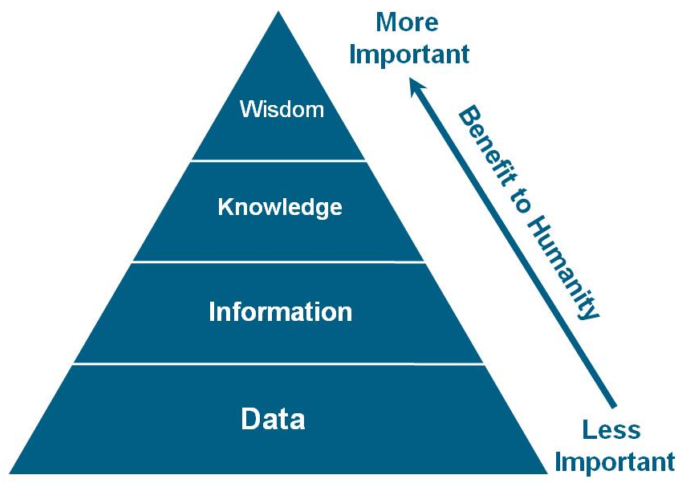
\includegraphics[width=\textwidth]{wkid}
			\fonte{\citetexto{Cisco2011}}
		\end{minipage}
	\end{figure}
	
%TODO Medir & Otimizar (gestão de processos)
	decisoes em tempo real a partir de leituras de sensores
	alta resolução dos dados, possibilitando controle individual de recursos 
	(big data)
	
%TODO Relacionar com Big Data
	
	\citetexto{Cisco2011} estima que em 2015 haverão 25 bilhões de 
	dispositivos conectados a Internet e que apenas 5 anos depois, em 
	2020, este número chegará a casa de 50 bilhões.

\section{Desafios}

%TODO Tecnológicos: bateria, processamento, antenas, protocolos
%TODO Sociais: ética, privacidade (big brother)

\section{Oportunidades}

	IBM Smarter Planet
	HP?
	
	inteligencia por agregação de dados
	processos autonomos
	
	explicar as principais vantagens do uso de IoT nos seguintes contextos
	Industria
	Meio Ambiente
	Sociedade (governamental)
	depois identificar e exemplificar os Application Domains 
	\cite{Sundmaeker2010}


\chapter{Proposta para IoT}

	Abordar neste capítulo as necessidades específicas de IoT e suas 
	características.
	
	Apresentar as dificuldades (problemas) que levarão para as propostas
	de como resolvê-las com as extensões ao protocolo.
	
	
	\section{Multicast}
		
		Propor o uso de multicast para enviar diversos comandos aos objetos
		disponíveis na rede.
		
		
	\section{Tageamento de Objetos}
		
		Propor um sistema para tagear objetos com base em características
		arbitrárias definidas pelo fabricante e pelo usuário.
		
		Quero enviar este comando para todos os objetos elétricos, para
		todos que estão na cozinha, para todos os sensores...
		
		
	\section{Compressão de Headers}
		
		Conforme feito por \cite{Choi2009}
		
		
	\section{Compressão de Dados}
		
		No caso do SNMP compressão das PDUs conforme \cite{Choi2009}
		
		
	% DESPRIORIZAR PORQUE É MUITO IGUAL E IMPORTANTE NO OUTRO ARTIGO
	\section{Requests Periódicos}
		
		Configurar uma mensagem que faz com que os clientes enviem
		dados de forma periódica para o server, evitando a necessidade
		de realizar pooling para obter informações.
		\cite{Choi2009}
		
		
%cronograma revisado
%metodologia revisada
%considerações finais
\chapter{Planejamento da Implementação}

\begin{verbatim}
aubinMIB
  - TagManager
    > Listar
    > Adicionar
    > Remover
  - TagDB
    - Tipo
      - Eletrônico
        > Estado (on / off)
        > Voltagem
        > Consumo
      - Áudio
        > Volume
      - Vídeo
        > Width
        > Height
        > Cores
      - Iluminação
        > Luminosidade %
        > Cor
    - Localização
      - GPS
        > Latitude
        > Longitude
      - Domiciliar
        - Sala
        - Quarto
        - Cozinha
\end{verbatim}

Manager precisa saber todas as tags de cada elemento pra conseguir fazer 
consultas por tag. Criar uma "resource" que notifica o manager das alterações 
nas tags (publish/subscribe) do COAP. Senão corre o risco do manager ficar com 
um estado desatualizado / inconsistente.

No caso do COAP os OIDs são traduzidos para resources, podendo ficar do tipo: 

\url{coap://192.168.1.15/snmp/tags/tipo/eletronico/estado}

tais resources recebem comandos RESTful (GET, POST, PUT, DELETE). Por exemplo, 
para desligar e ligar um objeto enviaria um request do tipo:

\url{POST(0) coap://192.168.1.15/snmp/tags/tipo/eletronico/estado}

\url{POST(1) coap://192.168.1.15/snmp/tags/tipo/eletronico/estado}

Adicionalmente, para reduzir o overhead poderia tentar criar um "alias" para 
as resources, tornando duas urls equivalentes, por exemplo:

\url{coap://192.168.1.15/snmp/tags/tipo/eletronico/estado}

\url{coap://192.168.1.15/snmp/tags/2/1/1}

	%TODO cronograma
	
	%TODO Diagrama de blocos entre dispositivos e gerente com as trocas de 
	%mensagens
	
	%TODO Como avaliar: Quantidade / tamanho das mensagens, tempos de 
	%resposta e processamento, consumo de recursos (pouco importante)
	

	Documentar o processo de implementação\ldots
	
	
	
	
%=======================================================================
% Referências
%=======================================================================
%TODO Revisar completeza dos dados
\bibliography{library}


%=======================================================================
% Exemplo de Apêndice
% O Apêndice é utilizado para apresentar material complementar elaborado
% pelo próprio autor.  Deve seguir as mesmas regras de formatação do
% corpo principal do documento.
%=======================================================================
%\appendix
%\chapter{Informações Complementares}
%
%O Apêndice é utilizado para apresentar material complementar elaborado
%pelo próprio autor.  Deve seguir as mesmas regras de formatação do
%corpo principal do documento.


%=======================================================================
% Exemplo de Anexo
% O Anexo é utilizado para a ``inclusão de materiais não elaborados pelo
% próprio autor, como cópias de artigos, manuais, folders, balancetes, etc.
% e não precisam estar em conformidade com o modelo''.
%=======================================================================
%\annex
%\chapter{Artigos Publicados}
%
%O Anexo é utilizado para a ``inclusão de materiais não elaborados pelo
%próprio autor, como cópias de artigos, manuais, folders, balancetes, etc.
%e não precisam estar em conformidade com o modelo''.


\end{document}
